\documentclass[paper=a4, fontsize=11pt]{scrartcl}
\usepackage[T1]{fontenc}
\usepackage[utf8]{inputenc}
\usepackage{lmodern}
\usepackage{multirow}
\usepackage[table,xcdraw]{xcolor}
\usepackage[spanish]{babel}
\usepackage{cite}
\usepackage{amsmath,amsfonts,amsthm} % Math packages
\usepackage{graphics,graphicx, float} %para incluir imágenes y colocarlas
\usepackage[backref,colorlinks=true,linkcolor=black,urlcolor=blue,citecolor=blue]{hyperref} %Para crear enlaces en el pdf
\usepackage[noabbrev,spanish]{cleveref}
\usepackage{url}
\usepackage[shortlabels]{enumitem}
\usepackage{appendix}
\usepackage{eurosym}
\usepackage{epsfig}
\usepackage{caption}
\usepackage{subcaption}

\renewcommand{\appendixname}{Anexo}
\renewcommand{\appendixtocname}{Anexo}
\renewcommand{\appendixpagename}{Anexo}

\numberwithin{figure}{section} % Number figures within sections (i.e. 1.1, 1.2, 2.1, 2.2 instead of 1, 2, 3, 4)
\numberwithin{table}{section} % Number tables within sections (i.e. 1.1, 1.2, 2.1, 2.2 instead of 1, 2, 3, 4)
\newcommand{\horrule}[1]{\rule{\linewidth}{#1}} % Create horizontal rule command with 1 argument of height

\title{
    \normalfont \normalsize
    \textsc{{\bf Ingeniería de Servidores (2015-2016)} \\ Grado en Ingeniería Informática \\ Universidad de Granada} \\ [25pt] % Your university, school and/or department name(s)
    \horrule{0.5pt} \\[0.4cm] % Thin top horizontal rule
    \huge Memoria Práctica 5 \\ % The assignment title
    \horrule{2pt} \\[0.5cm] % Thick bottom horizontal rule
}
\author{Antonio de la Vega Jiménez }

%*************************************************************


\begin{document}

\maketitle % Muestra el Título
\newpage %inserta un salto de página
\tableofcontents % para generar el índice de contenidos
\listoffigures
\listoftables
\newpage

%*************************************************************

\section{Instalación de servicios y configuraciones}

\subsection{yum}
%***********************************************
%    CUESTIÓN 1
%***********************************************
\subsubsection{Cuestión 1}
\textit{Liste los argumentos de yum necesarios para instalar, buscar y eliminar paquetes.}
\newline

Los argumentos necesarios son: \cite{manyum}
\begin{itemize}
  \item Instalar: \texttt{yum install nombrePaquete}
  \item Buscar: \texttt{yum search nombre}
  \item Eliminar: \texttt{yum remove nombrePaquete o yum erase nombrePaquete}
\end{itemize}


%***********************************************
%    CUESTIÓN 2
%***********************************************
\subsubsection{Cuestión 2}
\textit{Qué ha de hacer para que yum pueda tener acceso a Internet?(Pistas: archivo de configuración en /etc, proxy: stargate.ugr.es:3128). ¿Cómo añadimos un nuevo repositorio?}
\newline


\subsection{apt}
%***********************************************
%    CUESTIÓN 3
%***********************************************
\subsubsection{Cuestión 3}
\textit{Indique el comando para buscar un paquete en un repositorio y el correspondiente para instalarlo.}
\newline

Los comandos necesarios son: \cite{manapt1} \cite{manapt2}
\begin{itemize}
  \item Buscar: \texttt{apt-cache search expresiónRegular }
  \item Instalar: \texttt{apt-get install nombrePaquete}
\end{itemize}
%***********************************************
%    CUESTIÓN 4
%***********************************************
\subsubsection{Cuestión 4}
\textit{Indiqué qué ha modificado para que apt pueda acceder a los servidores de paquetes a través del proxy. ¿Cómo añadimos un nuevo repositorio?}
\newline


\subsection{Windows}

\subsection{OpenSuse}
%***********************************************
%    CUESTIÓN OP 1
%***********************************************
\subsubsection{Cuestión opcional 1}
\textit{¿Qué gestores utiliza OpenSuse?}
\newline
 
Los gestores de paquetes usados por OpenSuse son Zypper y Yast, aunque Yast realiza la misma tarea que Zypper pero con interfaz gráfica. \cite{os1} \cite{os2} \cite{os3}

\section{Gestión de los cortafuegos (firewalls)}
%***********************************************
%    CUESTIÓN 5
%***********************************************
\subsection{Cuestión 5}
\textit{¿Qué diferencia hay entre telnet y ssh?}
\newline

Tanto Telnet ( TELecommunication NETwork ) como SSH ( Secure Shell ) son protocolos de acceso remoto, la principal diferencia es la seguridad que ofrecen, Telnet no usa ningún tipo de cifrado en las comunicaciones, por lo que se pueden interceptar todos los datos de la comunicación ( incluyendo contraseñas ), debido a esto , su uso no es muy recomendable. SSH , al contrario que Telnet, si es un protocolo seguro, ya que todas las comunicaciones van cifradas.  \cite{sshtle}

%***********************************************
%    CUESTIÓN 6
%***********************************************
\subsection{Cuestión 6}
\textit{¿Para qué sirve la opción -X? Ejecute remotamente, es decir, desde la máquina anfitriona (si tiene Linux) o desde la otra máquina virtual, el comando gedit en una sesión abierta con ssh. ¿Qué ocurre?}
\newline

La opción -X de ssh sirve para que la aplicación se ejecute en el servidor remoto, pero la interfaz gráfica se visualice en el ordenador local ( X11 forwarding ). \cite{sshx} Al ejecutar gedit desde la terminal ssh, se muestra la aplicación como si se estuviese ejecutando en nuestro ordenador, pero en la ventana se indica que se esta ejecutando en otro ordenador ( on Ubuntu) Figura \ref{fig1}. 

\begin{figure}[H]
    \begin{center}
    \advance\leftskip-2.5cm
        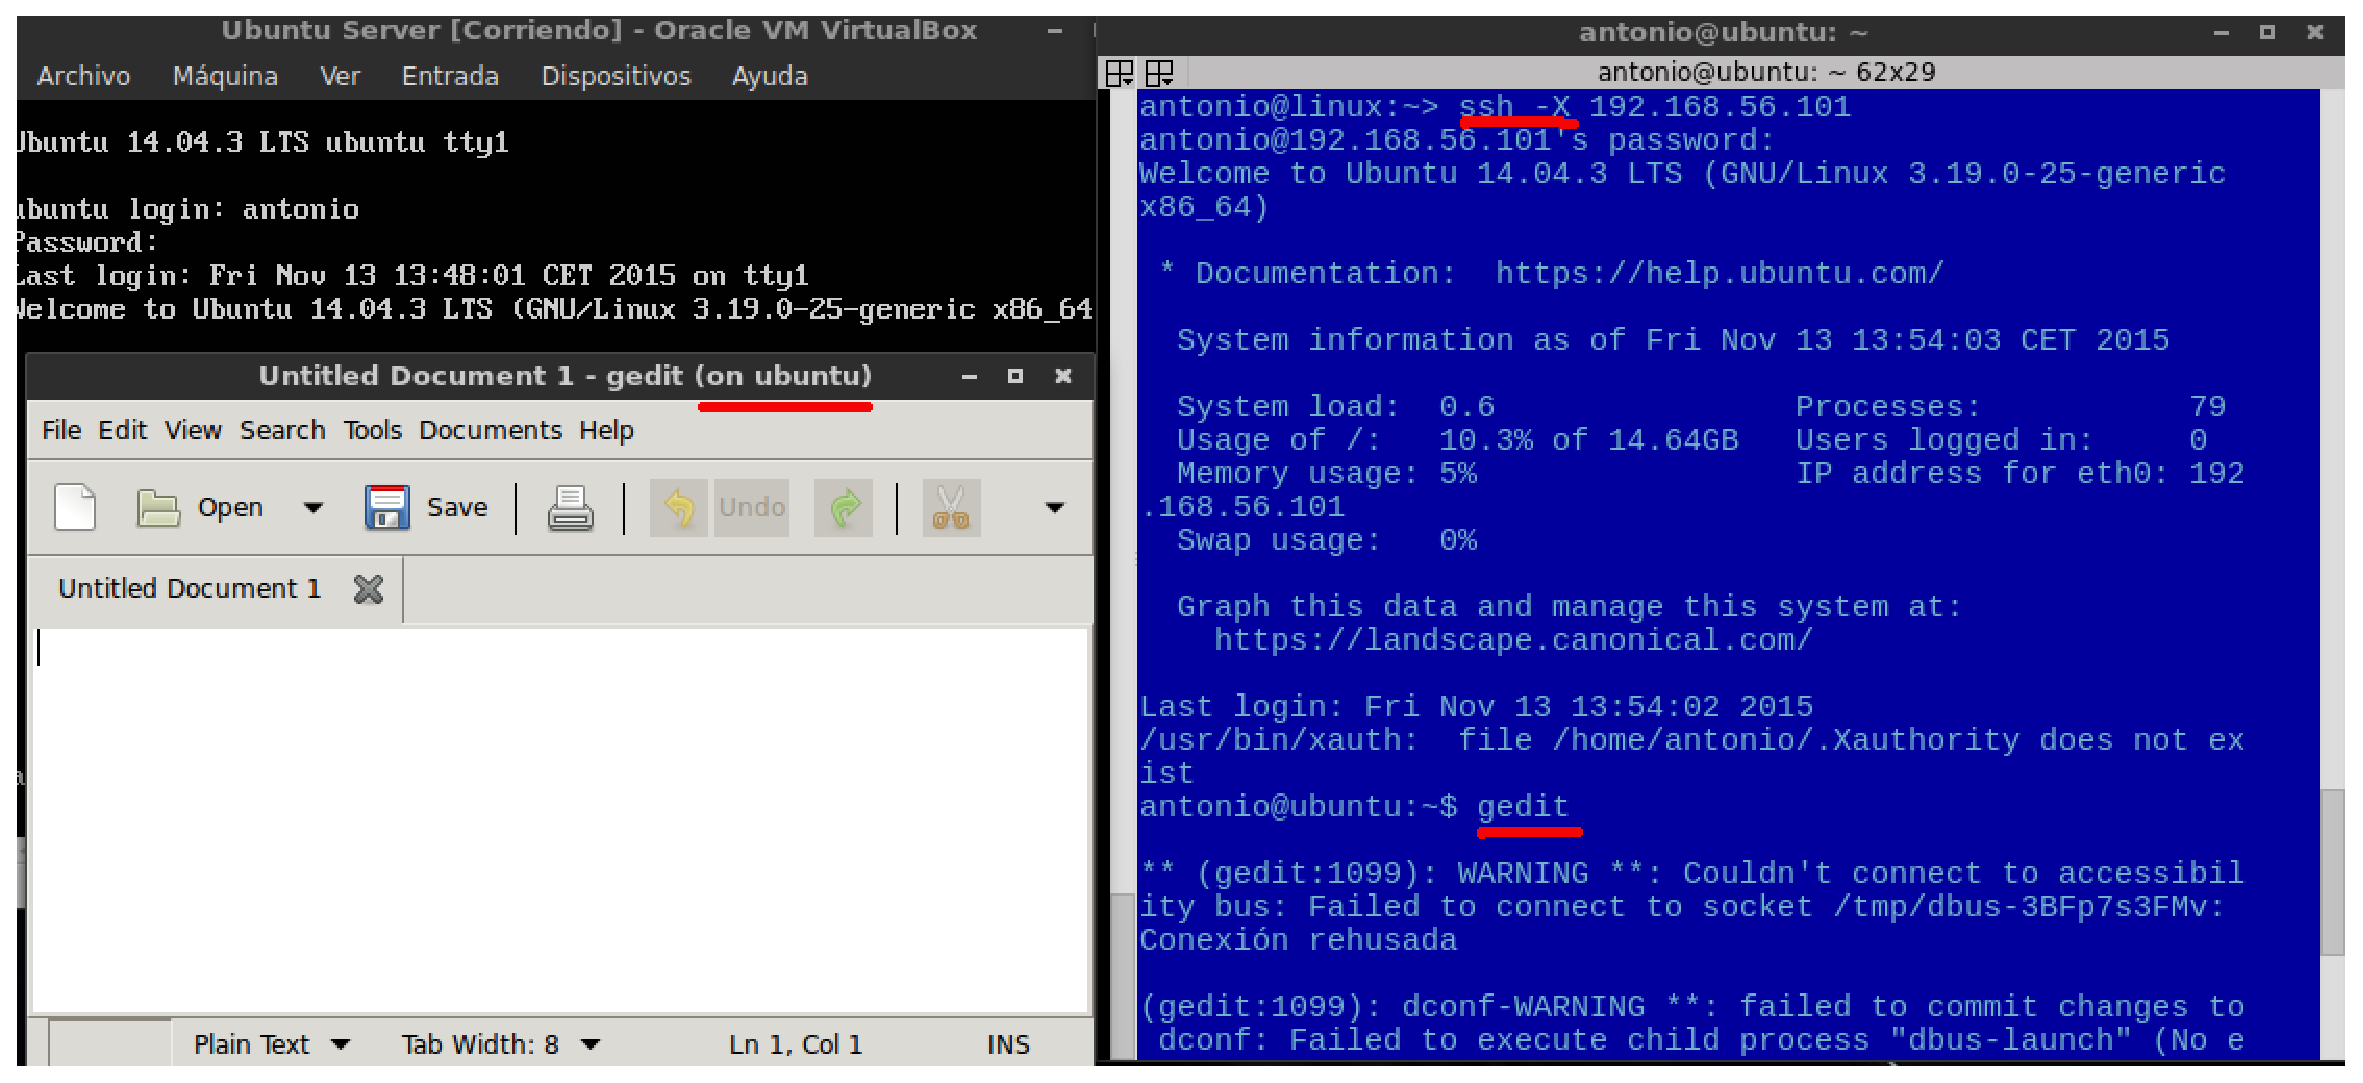
\includegraphics[scale=0.5]{imagenes/img1.eps}
        \caption{En esta imagen se muestra el resultado de ejecutar ssh con la opcción -X. Como se puede ver, en la aplicacion gedit se indica que la aplicación no esta siendo ejecutada en la máquina local, si no que se esta ejecutando en Ubuntu.}
        \label{fig1}
    \end{center}
\end{figure}


%***********************************************
%    CUESTIÓN 7
%***********************************************
\subsection{Cuestión 7}
\textit{Muestre la secuencia de comandos y las modificaciones a los archivos correspondientes para permitir acceder a la consola remota sin introducir la contraseña. (Pistas: ssh-keygen, ssh-copy-id).}
\newline

El proceso para permitir acceder a la consola sin introducir la contraseña consta de dos pasos: En primer lugar debemos crear una clave rsa y una carpeta para guardarla (en caso de que no exista ) , para ello hacemos uso de los comandos mostrados en la Figura \ref{fig2}. En segundo lugar debemos transferir la clave rsa que acabamos de crear al servidor remoto como se puede ver en la Figura \ref{fig3}, por último realizaremos una conexión ssh a la máquina remota y en caso de que no se nos pida una contraseña habremos verificado que la configuración se ha realizado correctamente ( Figura \ref{fig4}). \cite{passssh}

\begin{figure}[H]
    \begin{center}
        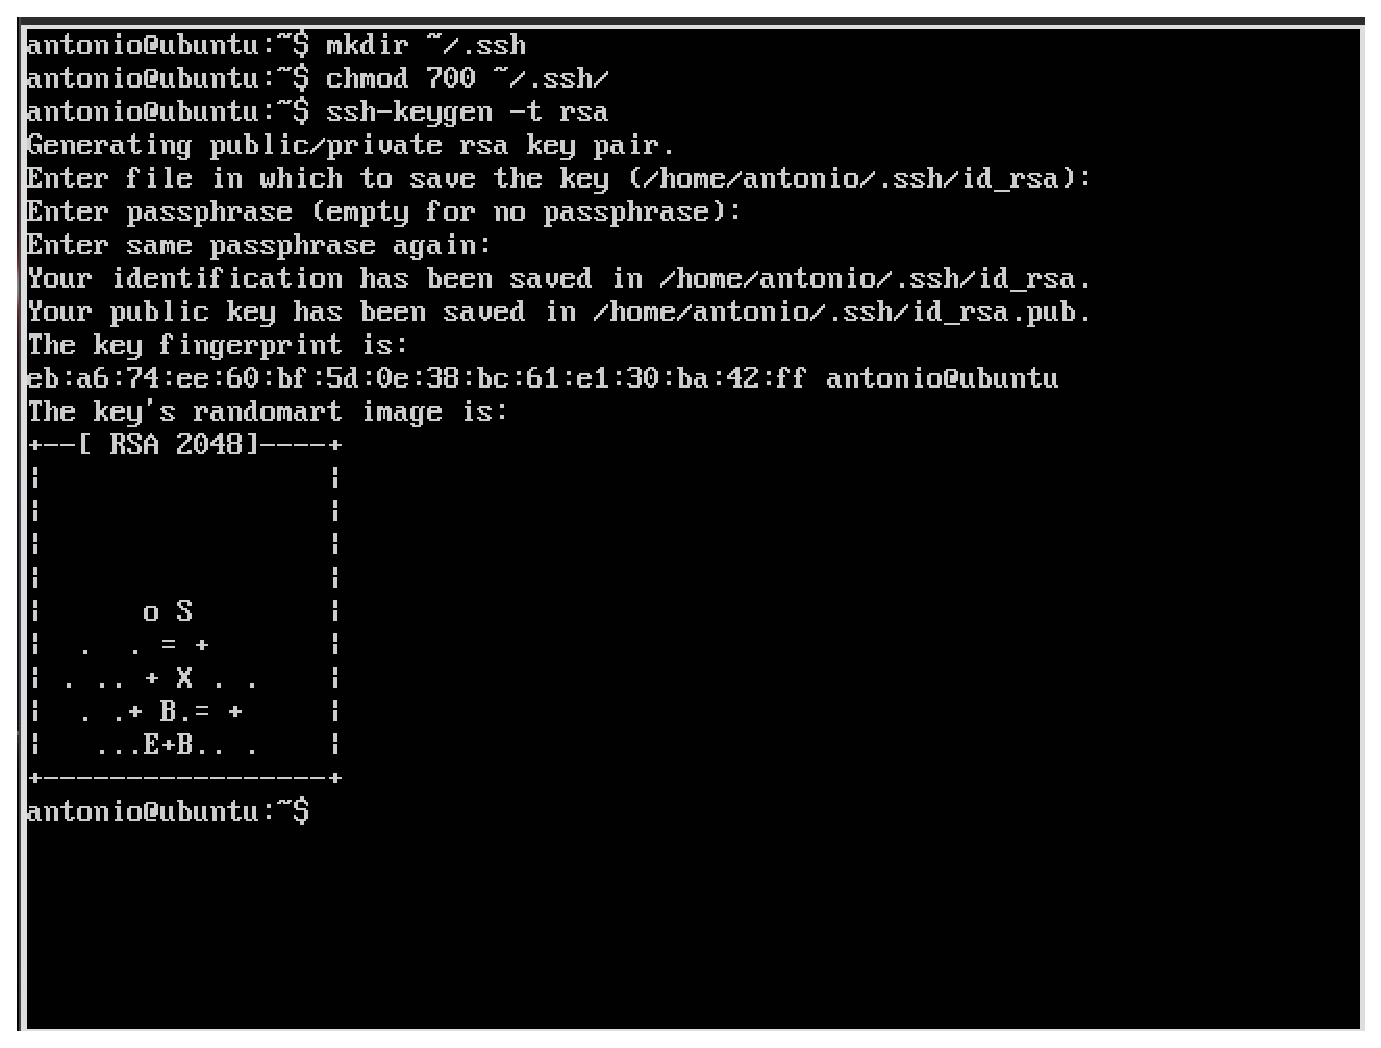
\includegraphics[scale=0.45]{imagenes/img2.eps}
        \caption{Secuencia de comandos necesaria para generar la clave rsa y la carpeta que guarda la clave.}
        \label{fig2}
    \end{center}
\end{figure}

\begin{figure}[H]
    \begin{center}
        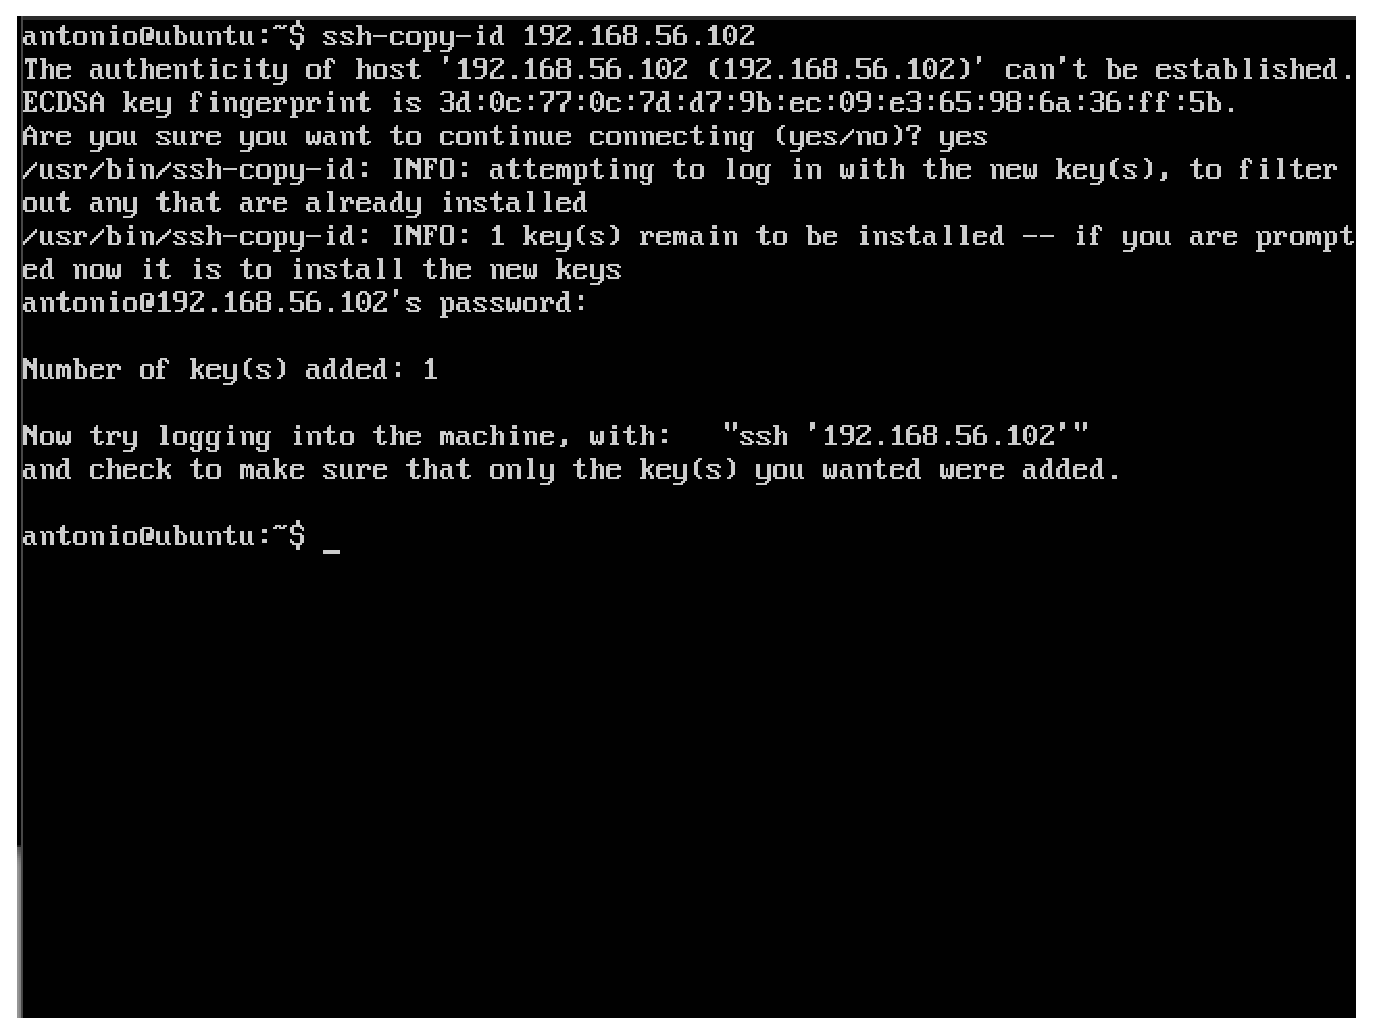
\includegraphics[scale=0.45]{imagenes/img3.eps}
        \caption{Comando para el traspaso de la clave de la máquina local a la máquina remota.}
        \label{fig3}
    \end{center}
\end{figure}

\begin{figure}[H]
    \begin{center}
        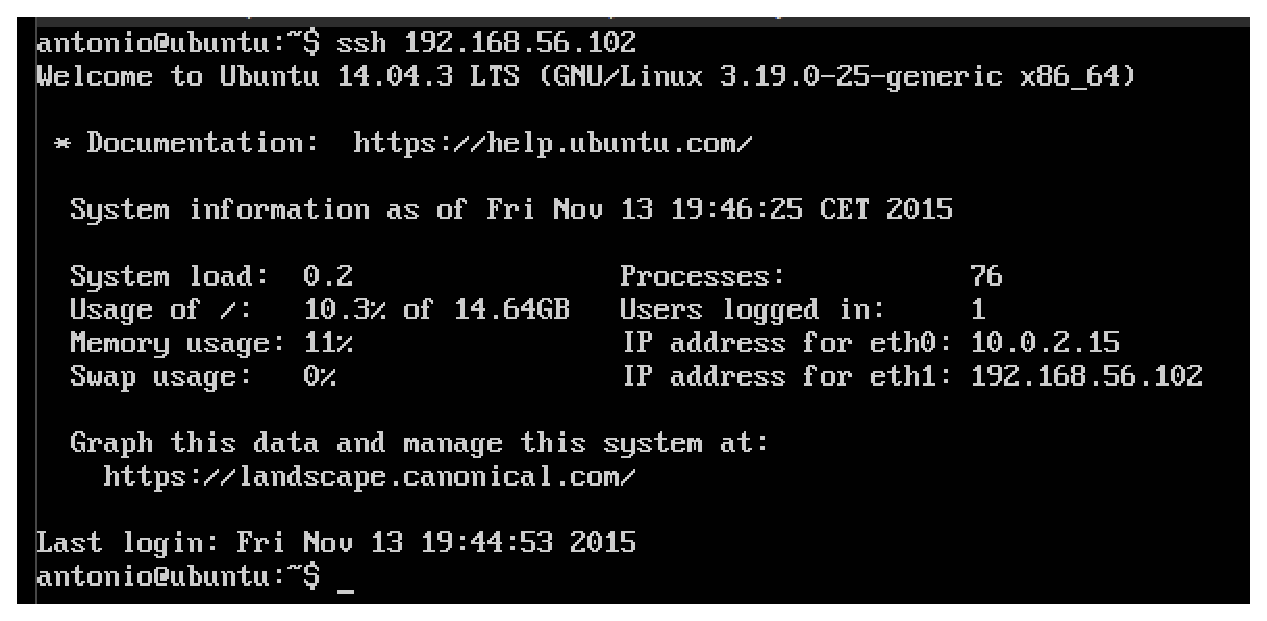
\includegraphics[scale=0.5]{imagenes/img4.eps}
        \caption{Comprobación de que podemos realizar una conexión ssh sin necesidad de introducir contraseña.}
        \label{fig4}
    \end{center}
\end{figure}

%***********************************************
%    CUESTIÓN 8
%***********************************************
\subsection{Cuestión 8}
\textit{¿Qué archivo es el que contiene la configuración de sshd? ¿Qué parámetro hay que modificar para evitar que el usuario root acceda? Cambie el puerto por defecto y compruebe que puede acceder.}
\newline

La configuración de sshd ( SSH daemon ) se encuentra en el archivo sshd\_config que se encuentra en /etc/ssh/sshd\_config. El parámetro que hay que modificar para que root no pueda acceder es PermitRootLogin y establecerlo a no, para cambiar el puerto se debe modificar el parámetro Port, tras realizar estas modificaciones, es necesario reiniciar ssh para que tengan efecto, esto se pude realizar mediante la orden \texttt{sudo service ssh restart} ( Ver configuración en las Figuras \ref{fig5} \ref{fig6} y el funcionamiento tras cambiar el puerto en la Figura \ref{fig7} y la imposibilidad de entrar como root en la Figura \ref{fig8} ) \cite{sshd}

\begin{figure}[H]
    \begin{center}
        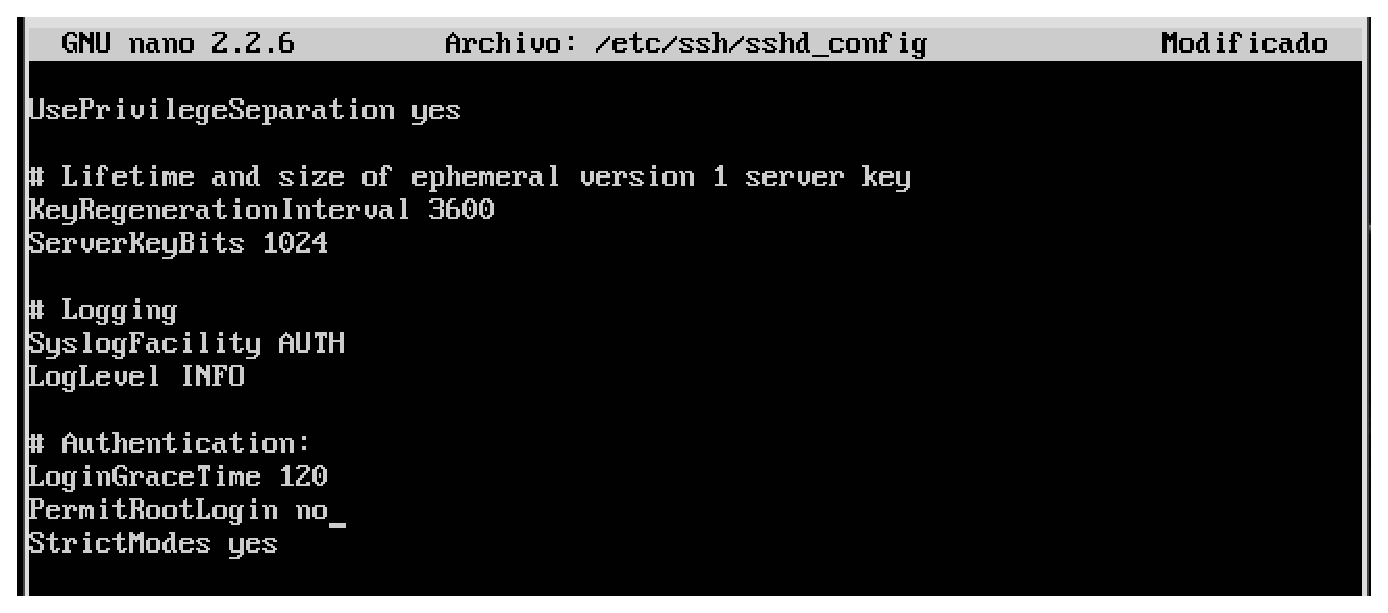
\includegraphics[scale=0.6]{imagenes/img5.eps}
        \caption{Configuracion par que root no pueda acceder (PermitRootLogin no).}
        \label{fig5}
    \end{center}
\end{figure}

\begin{figure}[H]
    \begin{center}
        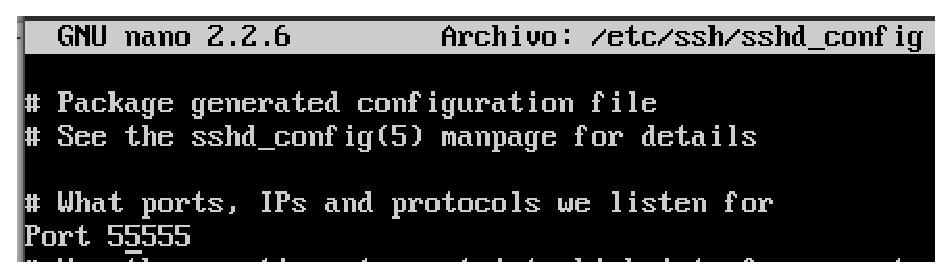
\includegraphics[scale=0.7]{imagenes/img7.eps}
        \caption{Cambio del puerto 22 establecido por defecto en ssh al puerto 55555.}
        \label{fig6}
    \end{center}
\end{figure}

\begin{figure}[H]
    \begin{center}
        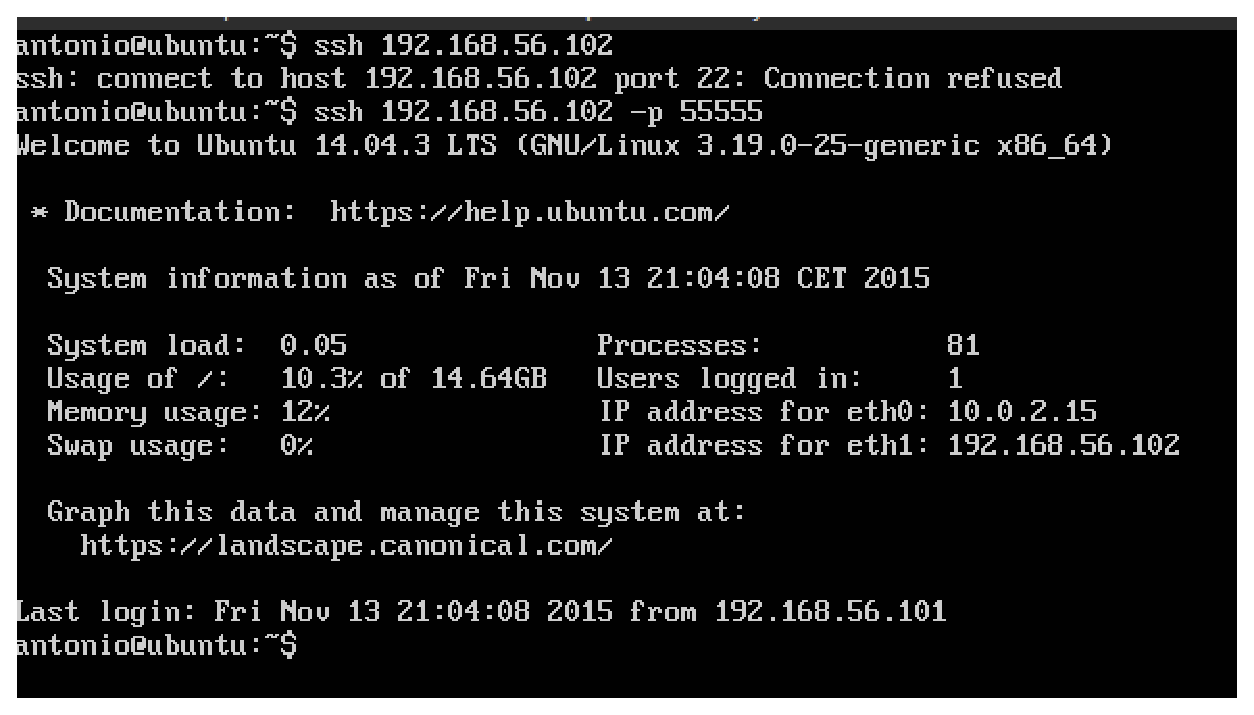
\includegraphics[scale=0.6]{imagenes/img6.eps}
        \caption{Comprobación de que el nuevo puerto ssh es el puerto 55555.}
        \label{fig7}
    \end{center}
\end{figure}

\begin{figure}[H]
    \begin{center}
        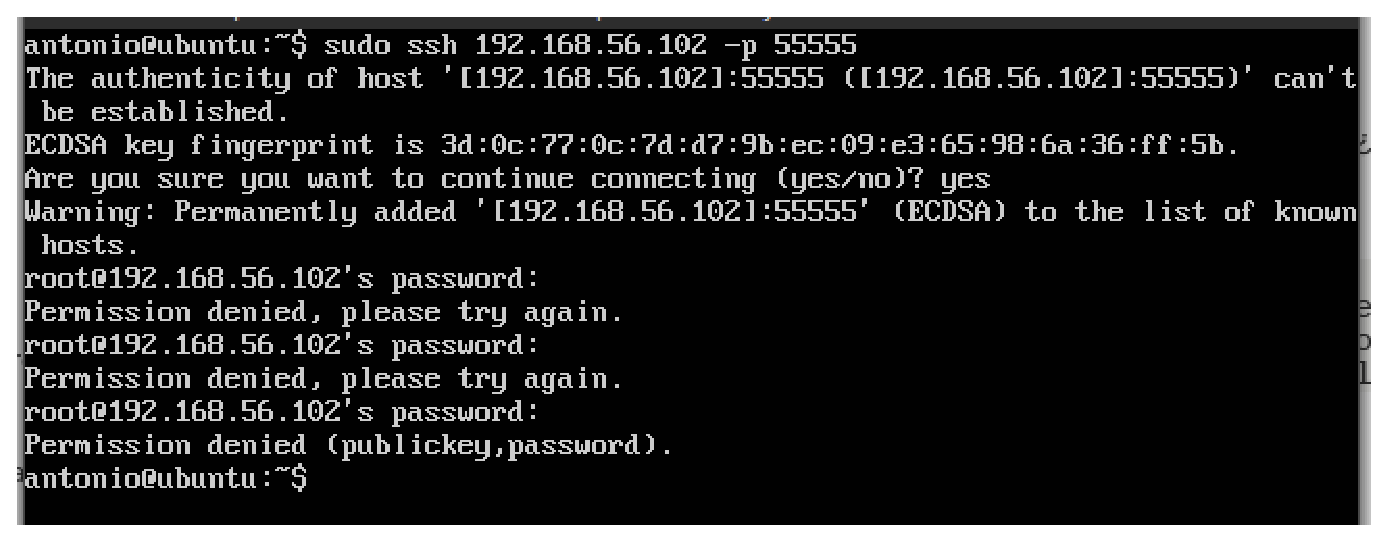
\includegraphics[scale=0.6]{imagenes/img8.eps}
        \caption{Comprobación de que no es posible acceder con el usuario root.}
        \label{fig8}
    \end{center}
\end{figure}

%***********************************************
%    CUESTIÓN 9
%***********************************************
\subsection{Cuestión 9}
\textit{Indique si es necesario reiniciar el servicio ¿Cómo se reinicia un servicio en Ubuntu? ¿y en CentOS? Muestre la secuencia de comandos para hacerlo.}
\newline

En ubuntu un servicio se puede reiniciar de dos formas,de la forma tradicional \newline
 \texttt{ /etc/init.d/nombreServicio restart } o de haciendo uso de  Upstart \newline
 \texttt{service nombreServicio start}. \cite{rest1} En CentOS( y RedHat ) los servicios se reinician mediante la orden anterior o la orden
 \texttt{systemctl restart nombre.service}. \cite{rest2}

\subsubsection{Utilidades: screen y terminator}
%***********************************************
%    CUESTIÓN OP 2
%***********************************************
\paragraph{Cuestión opcional 2}
\textit{Instale y pruebe terminator. Con screen, pruebe su funcionamiento dejando sesiones ssh abiertas en el servidor y recuperándolas posteriormente.}
\newline

Para instalar terminator en OpenSuse se puede realizar como se indica en la Figura \ref{fig10} . Para mostrar el funcionamiento de screen he ejecutado \texttt{screen} (Figura \ref{fig12}, una vez ahí he ejecutado la orden top (Figura \ref{fig13}) y mediante la combinación \texttt{Ctrl+a+d} me he desconectado de la ejecución de top (Figura \ref{fig14} y para terminar haciendo uso de la orden \texttt{screen -r } he vuelto a conectarme con la terminal que estaba ejecutando top (Figura \ref{fig15}), con esto se muestra que aunque pierdas la conexión con una terminal, luego es posible recuperarla sin ningún tipo de problema. Este proceso se muestra en la Figura \ref{fig16}


\begin{figure}[H]
    \centering
    \begin{subfigure}[b]{0.55\textwidth}
        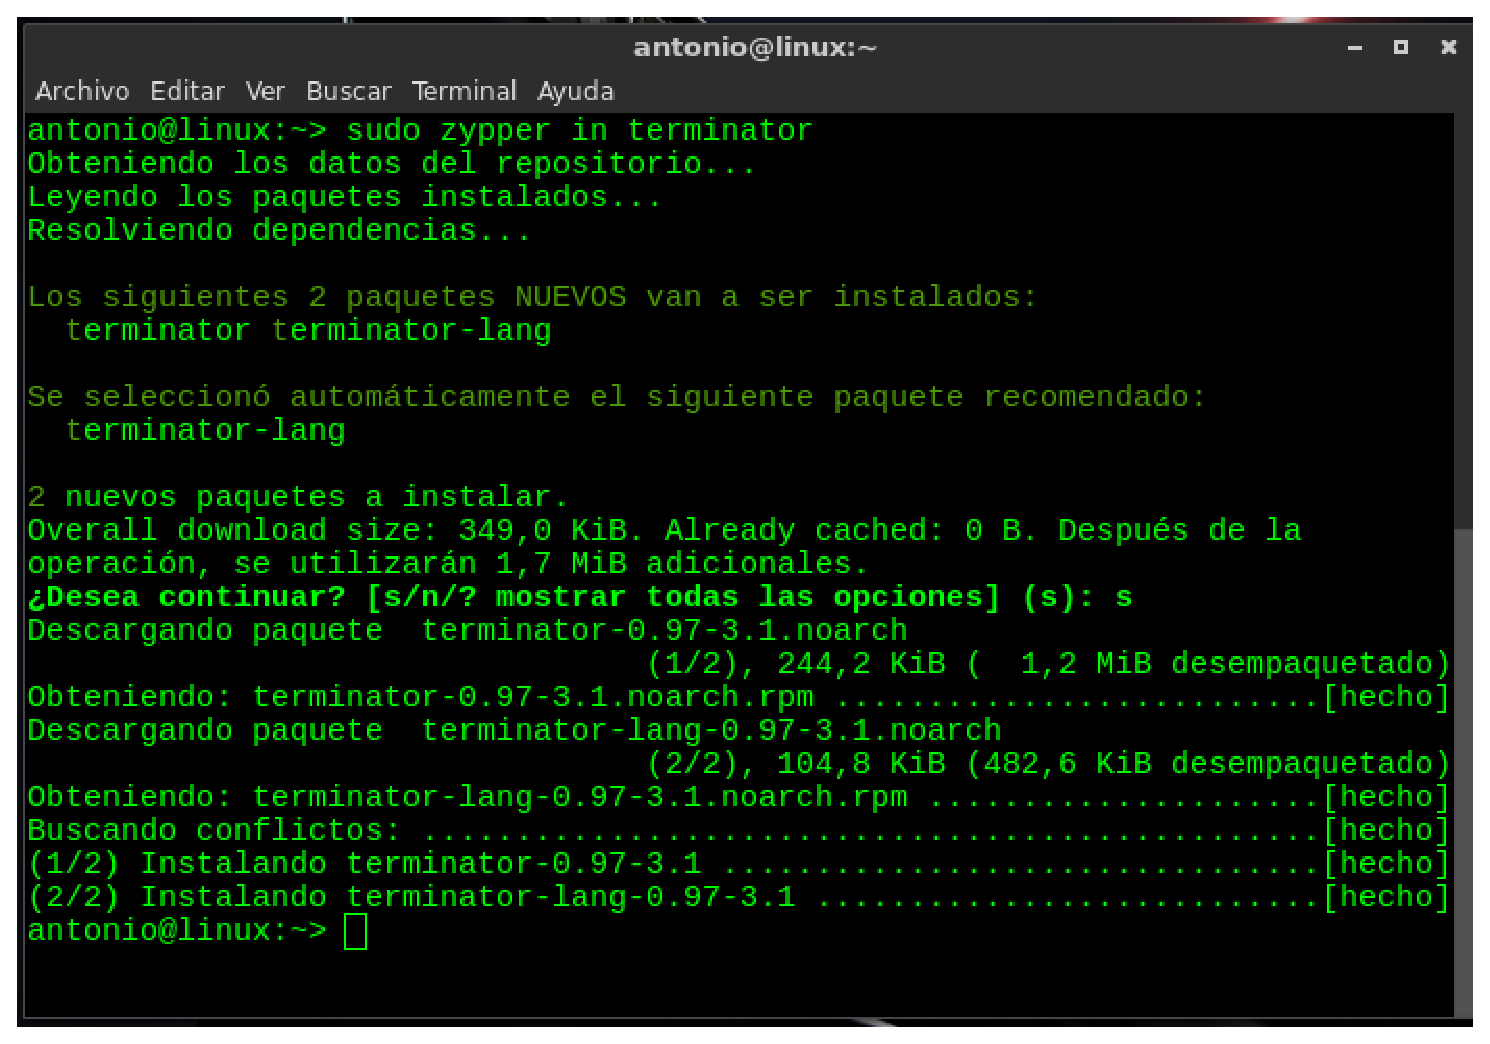
\includegraphics[width=\textwidth]{imagenes/img11.eps}
        \caption{Comando para la instalación de terminator.}
        \label{fig10}
    \end{subfigure}
    \begin{subfigure}[b]{0.4\textwidth}
        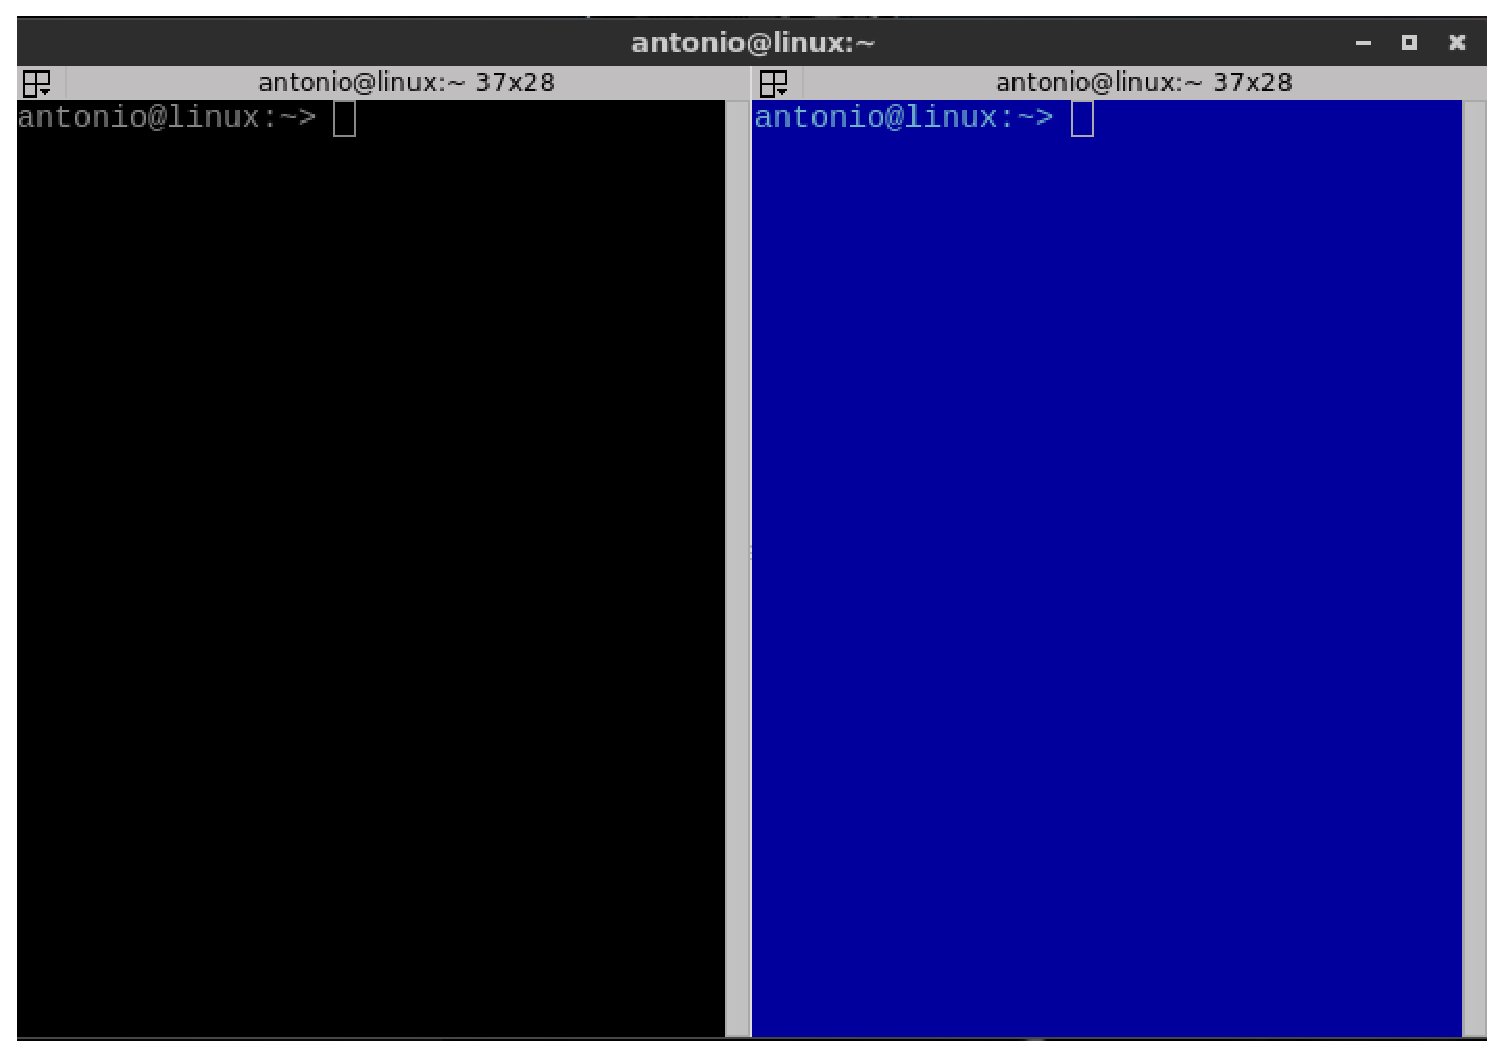
\includegraphics[width=\textwidth]{imagenes/img10.eps}
        \caption{Muestra de dos de las caracteristicas mas importantes de terminator,dividir la terminal y la creación distintos perfiles.}
        \label{fig11}
    \end{subfigure}
    \caption{Terminator}
\end{figure}



\begin{figure}[H] 
  \begin{subfigure}[b]{0.5\linewidth}
    \centering
    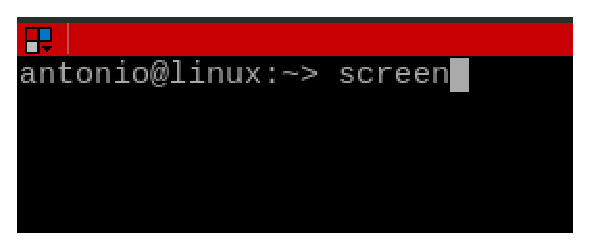
\includegraphics[width=0.75\linewidth]{imagenes/img12.eps} 
    \caption{Ejecución de screen.} 
    \label{fig12} 
    \vspace{4ex}
  \end{subfigure}%% 
  \begin{subfigure}[b]{0.5\linewidth}
    \centering
    
\includegraphics[width=0.75\linewidth]{imagenes/img13.eps} 
    \caption{Ejecución de top.} 
    \label{fig13} 
    \vspace{4ex}
  \end{subfigure} 
  \begin{subfigure}[b]{0.5\linewidth}
    \centering
    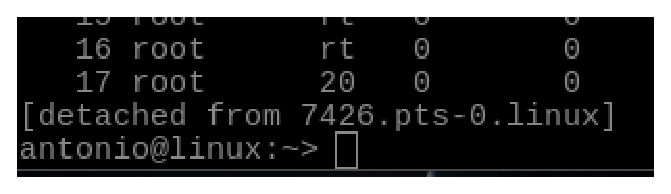
\includegraphics[width=0.75\linewidth]{imagenes/img14.eps} 
    \caption{Desconexión de la terminal con top.} 
    \label{fig14} 
  \end{subfigure}%%
  \begin{subfigure}[b]{0.5\linewidth}
    \centering
    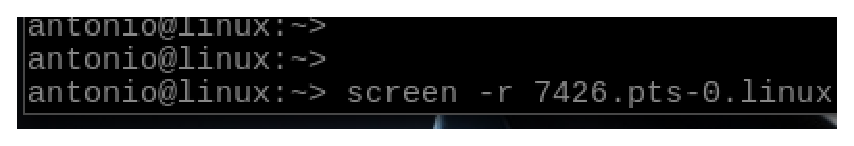
\includegraphics[width=0.75\linewidth]{imagenes/img15.eps} 
    \caption{Reconexión con top.} 
    \label{fig15} 
  \end{subfigure} 
  \caption{screen}
  \label{fig16} 
\end{figure}



\subsubsection{Un poco de seguridad: fail2ban}
%***********************************************
%    CUESTIÓN OP 3
%***********************************************
\paragraph{Cuestión opcional 3}
\textit{Instale el servicio y pruebe su funcionamiento.}


\section{Instalación del servicio de acceso remoto a la consola (Secure Shell)}


\section{Administración remota de windows}


\section{Instalación de un servidor Web básico}

\subsection{Instalación de Apache + MySQL (o MariaDB) + PHP (o Python) en Linux (LAMP)}

%***********************************************
%    CUESTIÓN 10
%***********************************************
\subsubsection{Cuestión 10}
\textit{Muestre los comandos que ha utilizado en Ubuntu Server y en CentOS (aunque en este último puede utilizar la GUI, en tal caso, realice capturas de pantalla)}
\newline

Para la instalación de LAMP en Ubuntu, he instalado los paquetes de  PHP, MySql y Apache de forma individual, haciendo uso de los siguientes comandos: \cite{l1 ,l2 ,l3} \newline

\hskip3.5cm \texttt{sudo apt-get install apache2 }

\hskip3.5cm \texttt{sudo apt-get install mysql-server }

\hskip3.5cm \texttt{sudo apt-get install php5 libapache2-mod-php5}

El funcionamiento del servidor se puede ver en la Figura \ref{fig17}

\begin{figure}[H]
    \begin{center}
        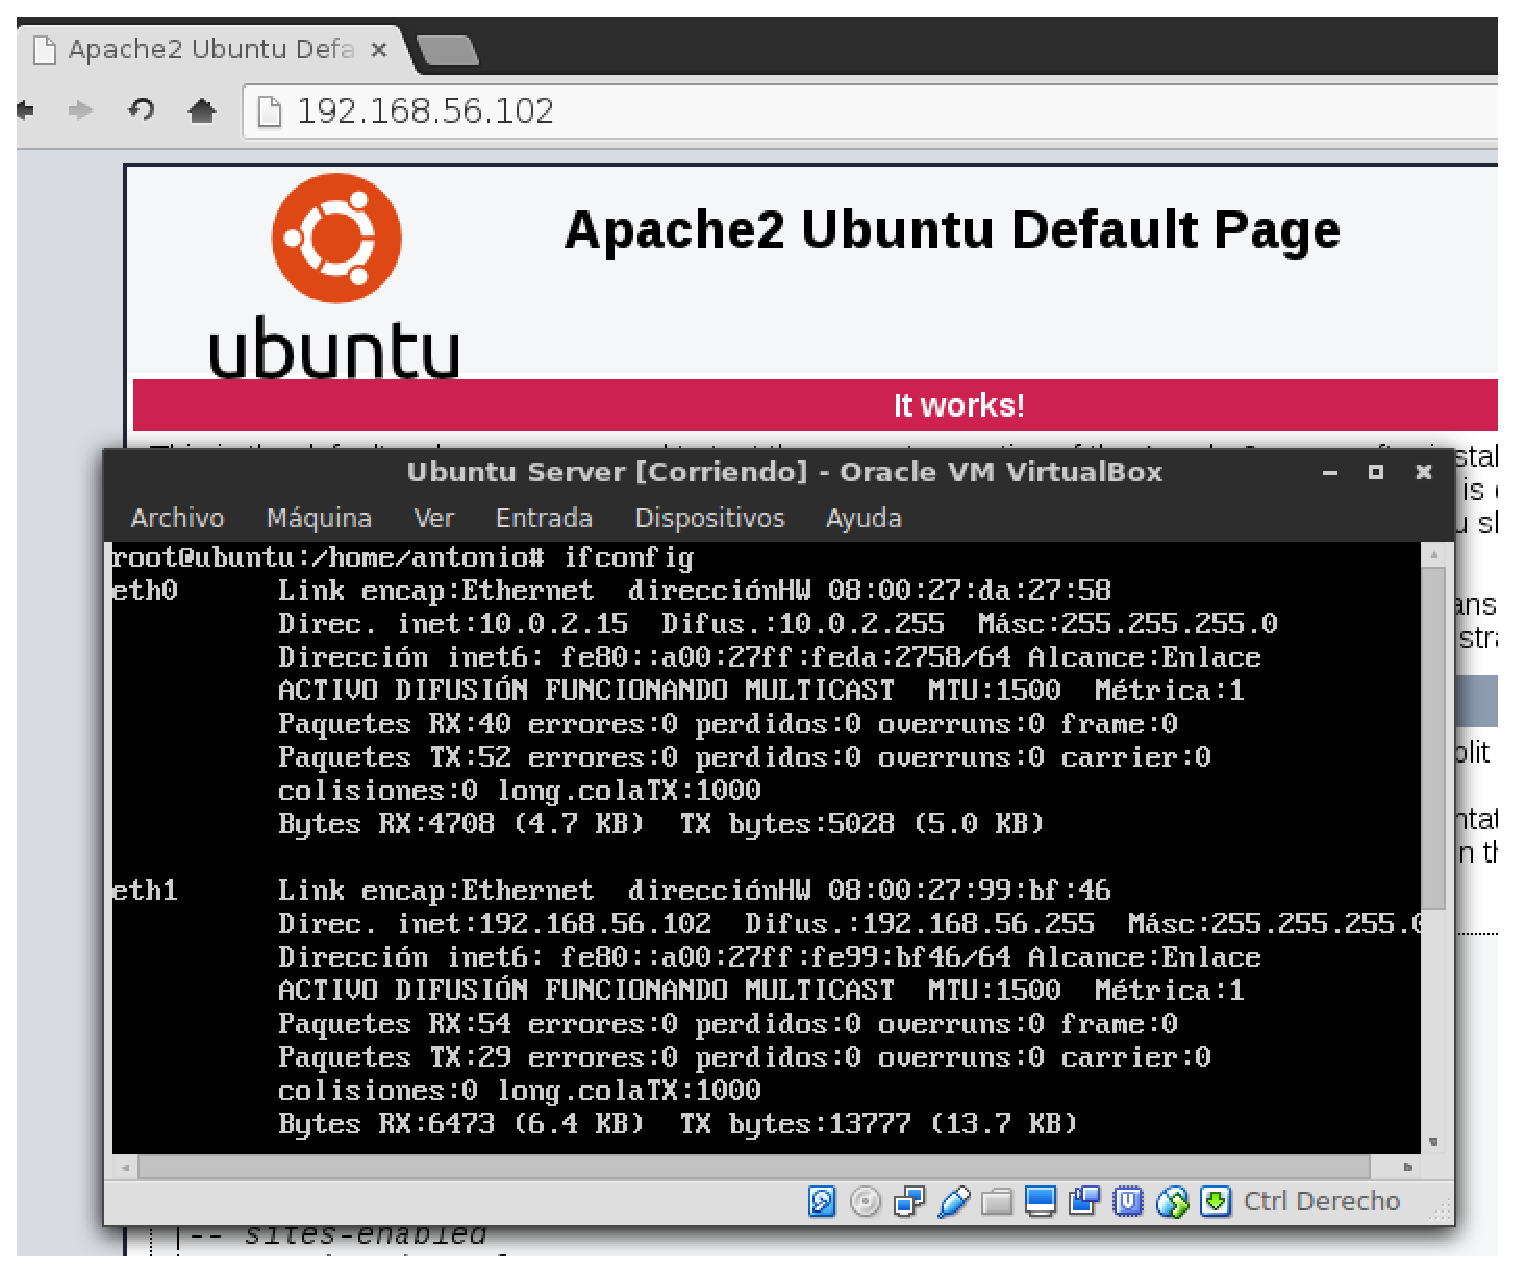
\includegraphics[scale=0.6]{imagenes/img17.eps}
        \caption{Ejecución del servidor LAMP.}
        \label{fig17}
    \end{center}
\end{figure}

Para la instalación de LAMP en CentOS, en primer lugar abrimos el gestor de software como se indica en la Figura \ref{fig18}, una vez hay buscamos e instalamos los paquetes \textbf{\texttt{httpd}} (apache), \textbf{\texttt{php}}, \textbf{\texttt{mysql-server}} y opcionalmente \textbf{\texttt{php-mysql}} (para usar MySQL desde PHP ) \cite{l4}. En la Figura \ref{fig19} se muestra el servidor en funcionamiento.

\begin{figure}[H]
    \begin{center}
        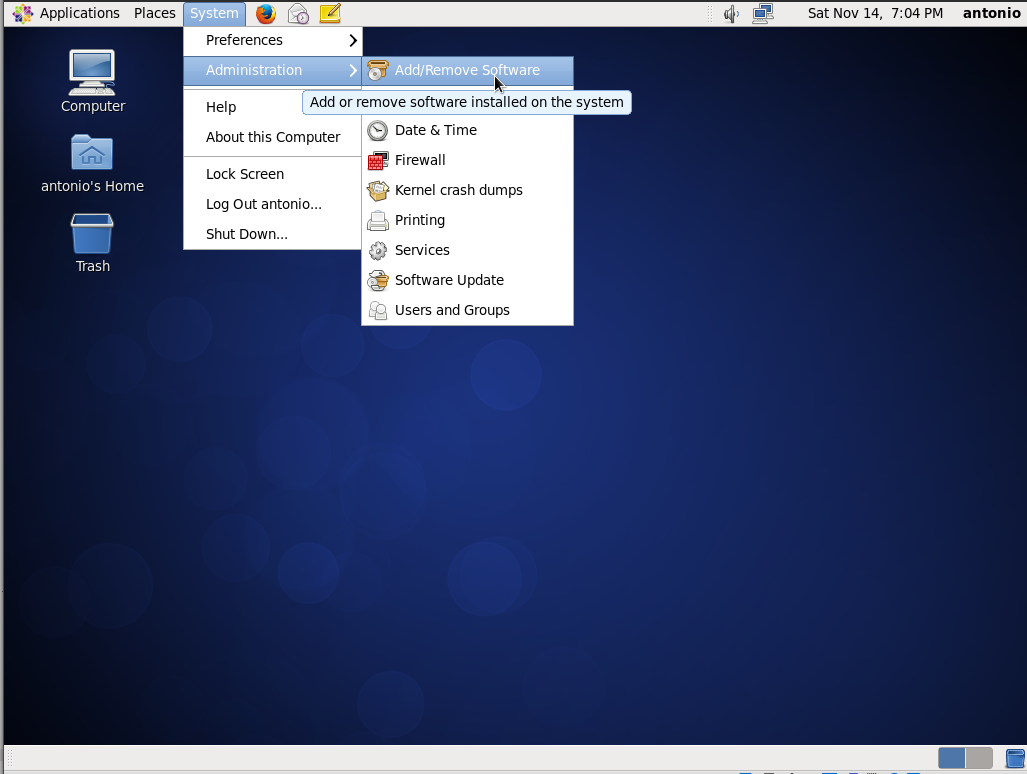
\includegraphics[scale=0.31]{imagenes/img18.eps}
        \caption{Acceso al gestor de software en Centos.}
        \label{fig18}
    \end{center}
\end{figure}

\begin{figure}[H]
    \begin{center}
        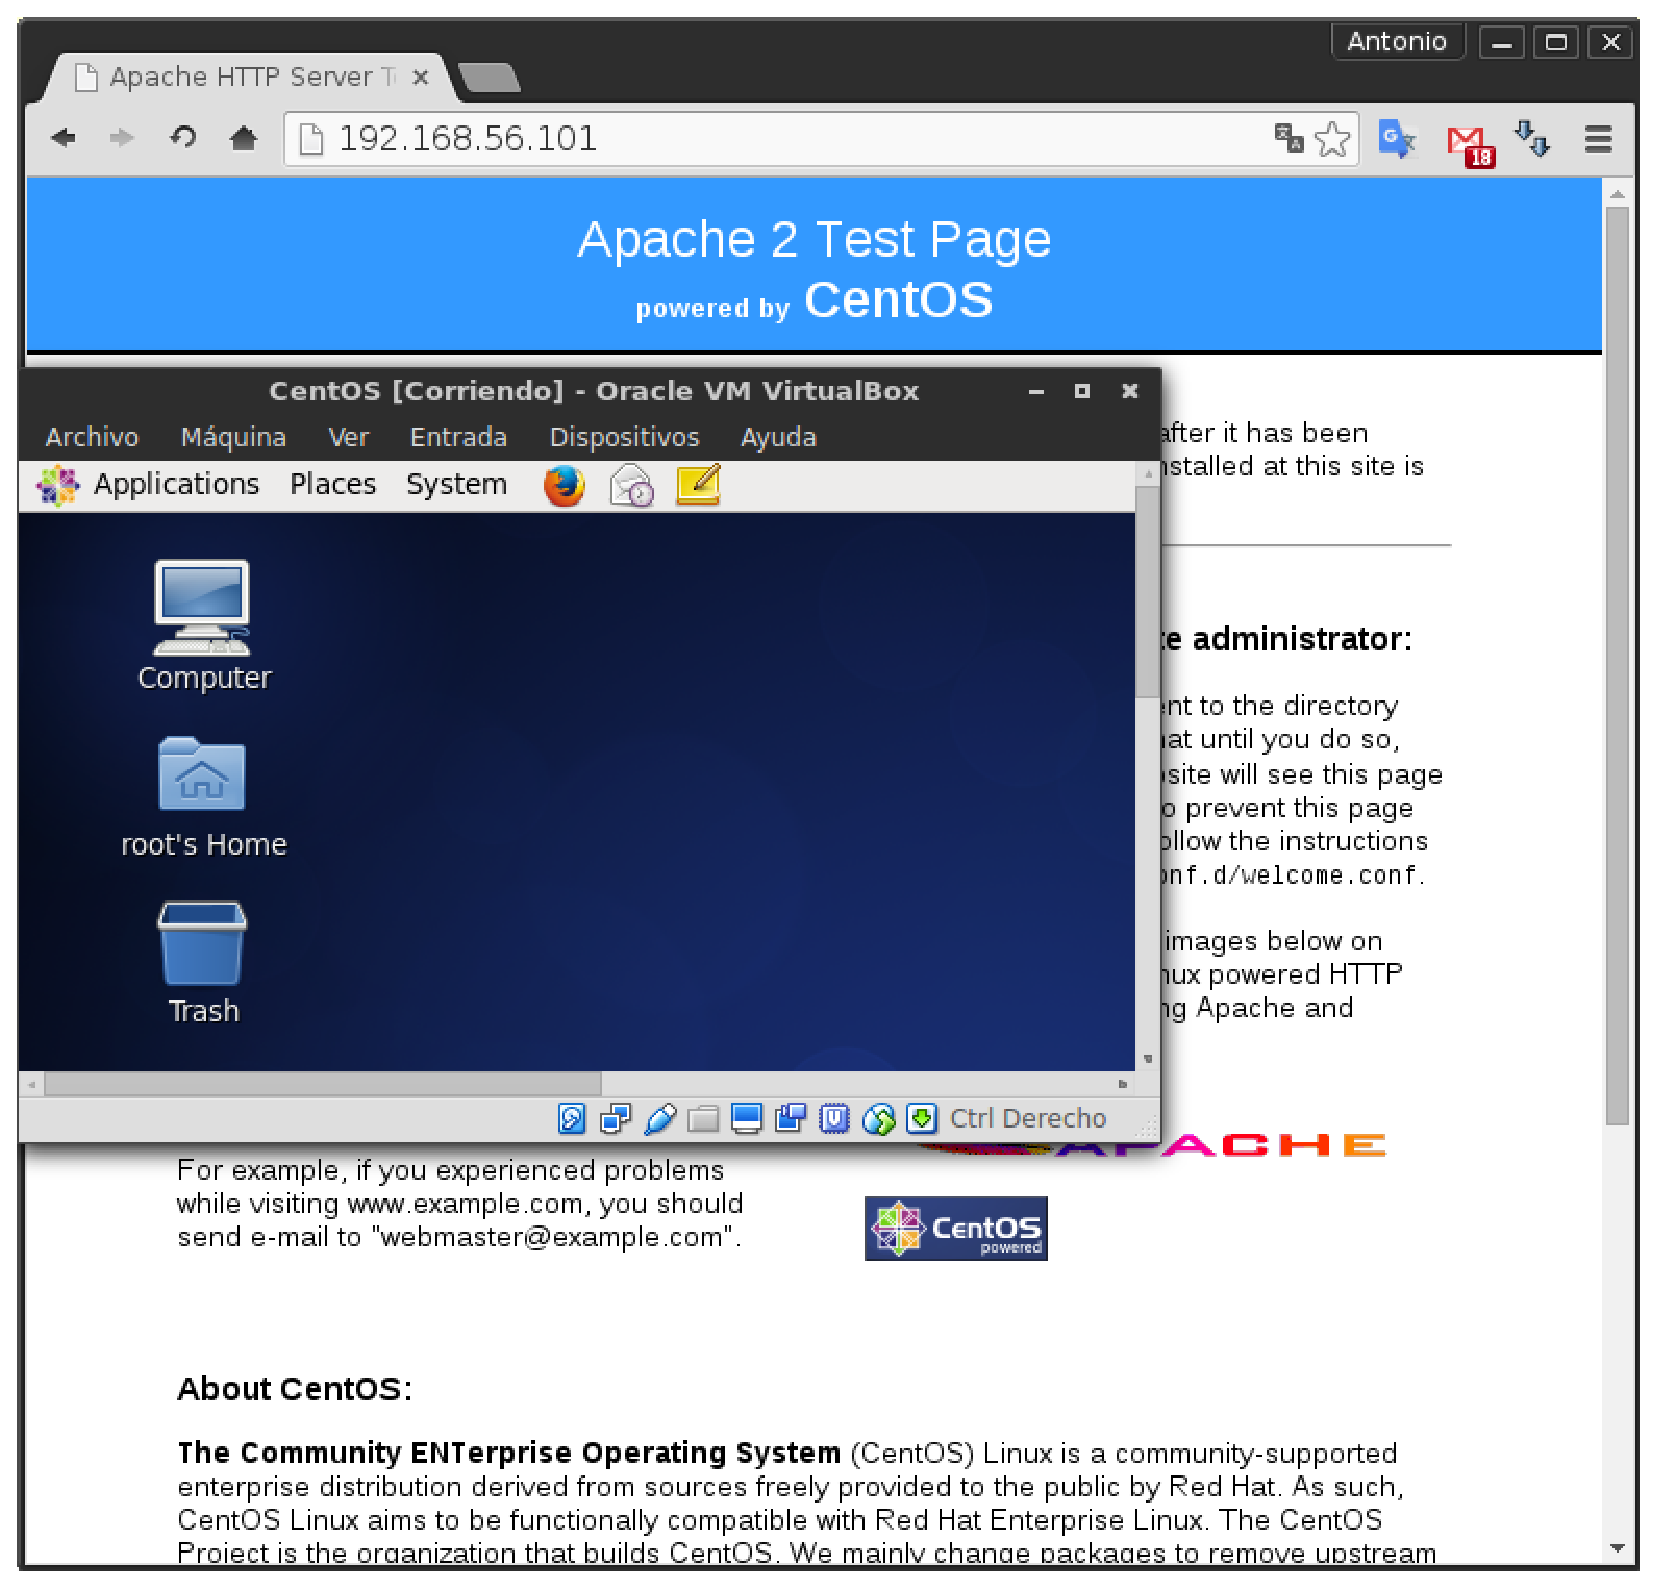
\includegraphics[scale=0.35]{imagenes/img19.eps}
        \caption{Servidor Apache en CentOS.}
        \label{fig19}
    \end{center}
\end{figure}

%***********************************************
%    CUESTIÓN 11
%***********************************************
\subsubsection{Cuestión 11}
\textit{Enumere otros servidores web y las páginas de sus proyectos (mínimo 3 sin considerar Apache, IIS ni nginx).}
\newline

Algunos servidores web son:
\begin{itemize}
  \item \textbf{Abyss Web Server: } \url{www.aprelium.com/abyssws/}
  \item \textbf{Hiawatha: } \url{www.hiawatha-webserver.org}
  \item \textbf{Lighttpd: } \url{www.lighttpd.net}
  \item \textbf{Cherokee: } \url{www.cherokee-project.com}

\end{itemize}
\subsection{Windows: IIS}
%***********************************************
%    CUESTIÓN 12
%***********************************************
\subsubsection{Cuestión 12}
\textit{Compruebe que el servicio está funcionando accediendo a la MV a través de la anfitriona.}
\newline

Tras realizar el proceso indicado en el punto 3.4.2 de la guia de la práctica para comprobar podemos  el funcionamiento de IIS introduciendo la IP del servidor en el navegador del host y ver que se accede a un web de IIS predeterminada, como se muestra en la Figura \ref{fig 20}.

\begin{figure}[H]
    \begin{center}
        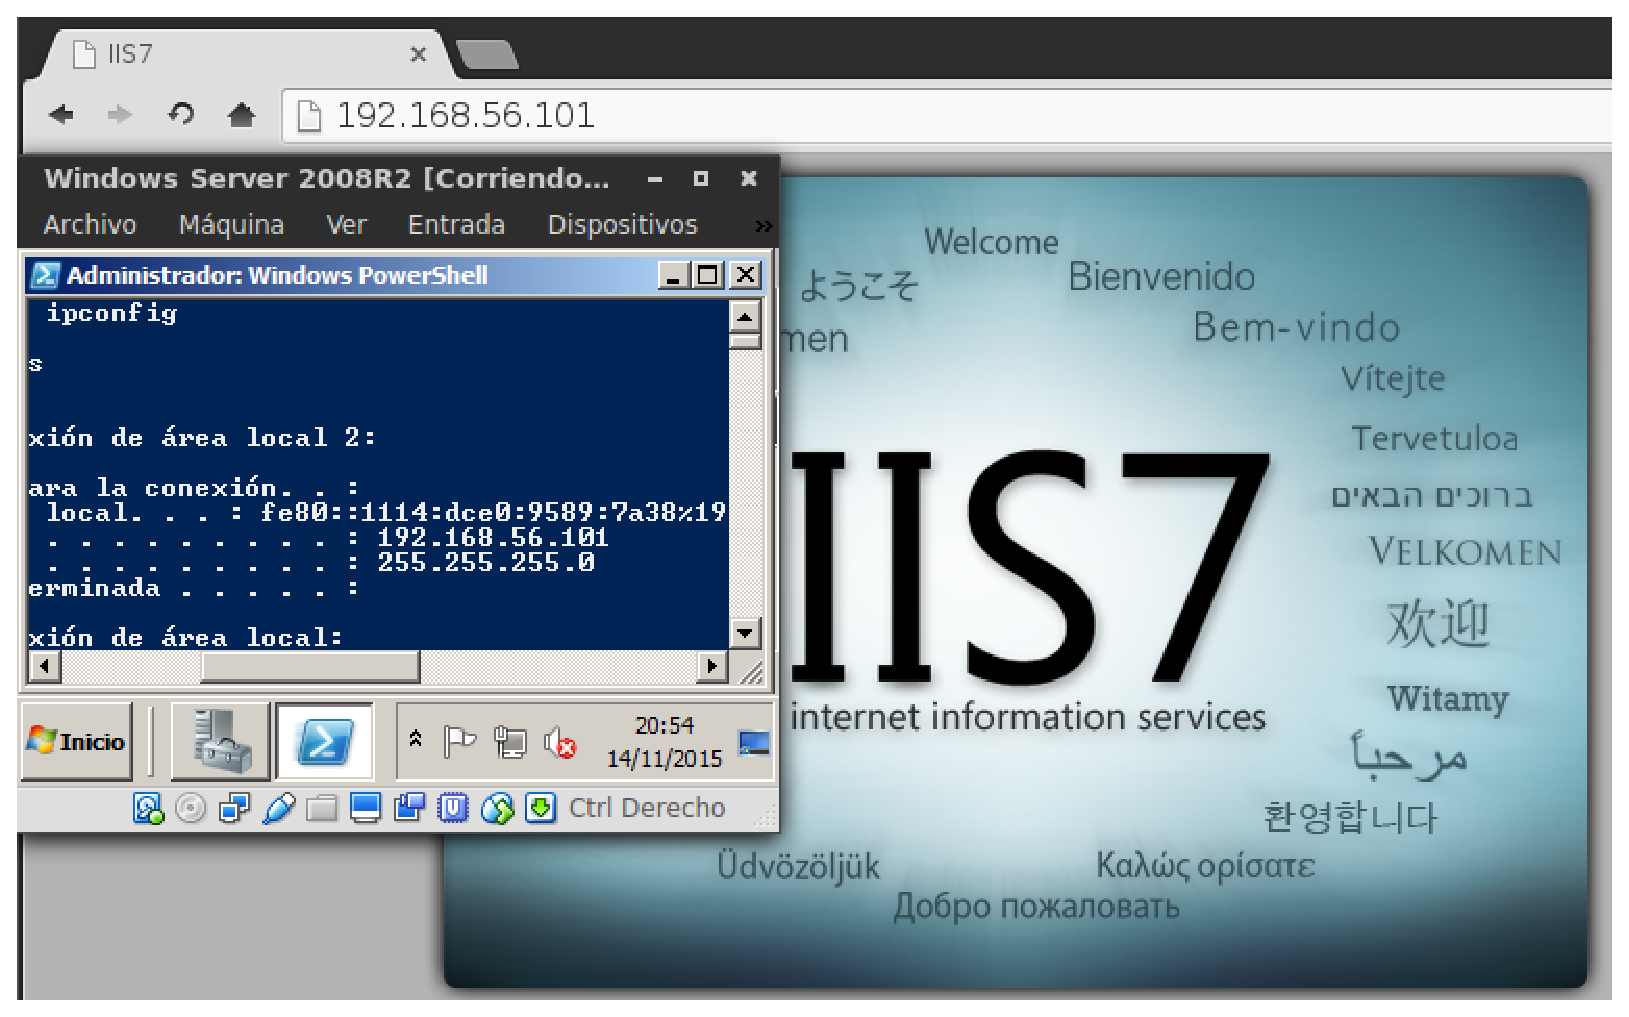
\includegraphics[scale=0.5]{imagenes/img20.eps}
        \caption{Muestra de que IIS se está ejecutando correctamente.}
        \label{fig20}
    \end{center}
\end{figure}

\subsection{Windows y otros servidores web}

\subsection{Java Servlets}
%***********************************************
%    CUESTIÓN OP 4
%***********************************************
\subsubsection{Cuestión opcional 4}
\textit{Realice la instalación de uno de estos dos “web containers” y pruebe su ejecución.}


\subsection{Otro tipo de Bases de datos}
%***********************************************
%    CUESTIÓN OP 5
%***********************************************
\subsubsection{Cuestión opcional 5}
\textit{Realice la instalación de MongoDB en alguna de sus máquinas virtuales. Cree una colección de documentos y haga una consulta sobre ellos. ( http://docs.mongodb.org/manual/installation/ )}


\section{Manteniendo los servicios actualizados}
%***********************************************
%    CUESTIÓN 13
%***********************************************
\subsection{Cuestión 13}
\textit{Muestre un ejemplo de uso del comando patch(p.ej. http://fedoraproject.org/wiki/VMWare)}
\newline


\section{Administración web}
%***********************************************
%    CUESTIÓN 14
%***********************************************
\subsection{Cuestión 14}
\textit{Realice la instalación de esta aplicación y pruebe a modificar algún parámetro de algún servicio. Muestre las capturas de pantalla pertinentes así como el proceso de instalación.}

%***********************************************
%    CUESTIÓN 15
%***********************************************
\subsection{Cuestión 15}
\textit{Instale phpMyAdmin, indique cómo lo ha realizado y muestre algunas capturas de pantalla.Configure PHP para poder importar BDs mayores de 8MiB (límite por defecto). Indique cómo ha realizado el proceso y muestre capturas de pantalla.}


\subsection{Más administradores:ISPCONFIG, DIRECTADMIN, CPANEL, PARALLELS PLESK,... }
%***********************************************
%    CUESTIÓN 16
%***********************************************
\subsubsection{Cuestión 16}
\textit{Viste al menos una de las webs de los software mencionados y pruebe las demos que ofrecen realizando capturas de pantalla y comentando qué está realizando.}


\section{Automatización de tareas con scripts}
\subsection{Shells}
%***********************************************
%    CUESTIÓN 17
%***********************************************
\subsubsection{Cuestión 17}
\textit{Ejecute los ejemplos de find, grep y escriba el script que haga uso de sed para cambiar la configuración de ssh y reiniciar el servicio.}

%***********************************************
%    CUESTIÓN OP6
%***********************************************
\subsubsection{Cuestión opcional 6}
\textit{Muestre un ejemplo de uso para awk.}


\subsection{PHP}
\subsection{Python}
%***********************************************
%    CUESTIÓN 18
%***********************************************
\subsubsection{Cuestión 18}
\textit{Escriba el script para cambiar el acceso a ssh usando PHP o Python.}


\subsection{Windows PowerShell}
%***********************************************
%    CUESTIÓN 19
%***********************************************
\subsubsection{Cuestión 19}
\textit{Abra una consola de Powershell y pruebe a parar un programa en ejecución (p.ej), realice capturas de pantalla y comente lo que muestra.}

\subsection{Más automatización}


%*************************************************************
\newpage
\bibliographystyle{ieeetr}
\bibliography{citas}

\end{document}
